        %%******************************************%%
        %%                                          %%
        %%        Modello di tesi di laurea         %%
        %%            di Andrea Giraldin            %%
        %%                                          %%
        %%             2 novembre 2012              %%
        %%                                          %%
        %%******************************************%%

\begin{document}
    \frontmatter
    \begin{titlepage}
    \begin{center}
        \begin{LARGE}
            \textbf{\myUni}\\
        \end{LARGE}

        \vspace{10pt}

        \begin{Large}
            \textsc{\myDepartment}\\
        \end{Large}

        \vspace{10pt}

        \begin{large}
            \textsc{\myFaculty}\\
        \end{large}

        \vspace{30pt}
        \begin{figure}[htbp]
            \centering
            
\includegraphics[height=6cm]{unipd-logo}
        \end{figure}
        \vspace{30pt}

        \begin{LARGE}
            \textbf{\myTitle}\\
        \end{LARGE}

        \vspace{10pt}

        \begin{large}
            \textsl{\myDegree}\\
        \end{large}

        \vspace{40pt}

        \begin{large}
            \begin{flushleft}
                \textit{Relatore}\\
                \vspace{5pt}
                \profTitle\ \myProf
            \end{flushleft}

            % You can tweak the spacing to have professor and student names on the same line
            % useful if the page is broken by a long thesis title and you need more space
            % \vspace{-52pt}

            \begin{flushright}
                \textit{Laureando}\\
                \vspace{5pt}
                \myName
            \end{flushright}
        \end{large}

        \vspace{40pt}

        \line(1, 0){338} \\
        \begin{normalsize}
            \textsc{Anno Accademico \myAA}
        \end{normalsize}
    \end{center}
\end{titlepage}

    \clearpage
\phantomsection
\thispagestyle{empty}

\hfill
\vfill

\noindent\myName: \textit{\myTitle,}
\myDegree,
\textcopyright\ \myTime.

    \cleardoublepage
\phantomsection
\thispagestyle{empty}
\pdfbookmark{Dedica}{Dedica}

\vspace*{3cm}

\begin{center}
    Feeling my way through the darkness\\
    Guided by a beating heart\\
    I can't tell where the journey will end\\
    But I know where to start \\ \medskip
    --- Avicii. \textit{Wake me up}
\end{center}

\medskip

\begin{center}
    Dedicato a me stesso
\end{center}

    \cleardoublepage
\phantomsection
\pdfbookmark{Sommario}{Sommario}
\begingroup
\let\clearpage\relax
\let\cleardoublepage\relax
\let\cleardoublepage\relax

\chapter*{Sommario}

Il presente documento descrive il lavoro svolto durante il periodo di stage, della durata di X ore, dal laureando Marco Brigo presso l'azienda Omicron Consulting Srl di Padova nel periodo che va dal 19 Giugno 2023 a X Agosto 2023.
L'obiettivo dello stage è lo sviluppo del lato back-end per un software di pianificazione delle risorse aziendali, verso determinati incarichi, utilizzato da chi di competenza in azienda.
La parte da me sviluppata permette di poter effettuare delle richieste di pianificazione di determinate figure professionali per lo svolgimento di specifici incarichi sotto determinati filtri.
L'attività si è svolta passando da uno studio preliminare delle tecnologie da utilizzare tramite esercitazioni e materiale fornito, passando per una progettazione dell'architettura e del database.
Infine....\\
...\\
Gli obbiettivi da raggiungere erano molteplici.\\
In primo luogo era richiesto lo sviluppo di ...
In secondo luogo era richiesta l'implementazione di un ...
Tale framework permette di registrare gli eventi di un controllore programmabile, quali segnali applicati
Terzo ed ultimo obbiettivo era l'integrazione ...

%\vfill

%\selectlanguage{english}
%\pdfbookmark{Abstract}{Abstract}
%\chapter*{Abstract}

%\selectlanguage{italian}

\endgroup

\vfill

    \cleardoublepage
\phantomsection
\pdfbookmark{Ringraziamenti}{ringraziamenti}

%\begin{flushright}{
%    \slshape
%    ``Feeling my way through the darkness, guided by a beating heart, I can't tell where the journey will end, but I know where to start.''} \\
%    \medskip
%    --- Wake me up, Avicii
%\end{flushright}


\bigskip

\begingroup
\let\clearpage\relax
\let\cleardoublepage\relax
\let\cleardoublepage\relax

\chapter*{Ringraziamenti}

\noindent \textit{Innanzitutto, vorrei esprimere la mia gratitudine al Prof. \myProf, relatore della mia tesi, per l'aiuto, i consigli e il sostegno fornitomi durante la stesura del lavoro.}\\

\noindent \textit{Ringrazio il mio tutor aziendale Antonio Fasolato per gli insegnamenti forniti con pazienza e dedizione, e desidero esprimere la mia gratitudine anche ai colleghi incontrati durante questo percorso, per tutti i momenti divertenti e gli aiuti che mi hanno dato.}\\

\noindent \textit{Desidero ringraziare con affetto i miei genitori e i parenti per il sostegno, il grande aiuto e la pazienza dimostrata in questi anni di studio, e per avermi sempre incoraggiato a dare il meglio di me.}\\

\noindent \textit{Ringrazio infine tutti gli amici che ho incontrato durante questi bellissimi anni di studio. In particolar modo ringrazio Michael e Fabio per tutte le avventure vissute, tutti gli esami affrontati insieme e le chiacchierate fatte dietro ad uno spritz.}\\
\bigskip


\noindent\textit{\myLocation, \myTime}
\hfill \myName

\endgroup

    \cleardoublepage
\pdfbookmark{\contentsname}{tableofcontents}
\setcounter{tocdepth}{2}
\tableofcontents
%\markboth{\contentsname}{\contentsname}
\clearpage

\begingroup
    \let\clearpage\relax
    \let\cleardoublepage\relax
    \let\cleardoublepage\relax

    % Figures list
    \phantomsection
    \pdfbookmark{\listfigurename}{lof}
    \listoffigures

    \vspace*{8ex}

    % Tables list
    \phantomsection
    \pdfbookmark{\listtablename}{lot}
    \listoftables

    \vspace*{8ex}
\endgroup

\cleardoublepage

    \cleardoublepage

    \mainmatter
    \chapter{Introduzione}
\label{cap:introduzione}
\section{Convenzioni tipografiche nel documento}
Durante la stesura del testo sono state adottate le seguenti convenzioni:
\begin{itemize}
\item la sezione del glossario contiene i termini ritenuti ambigui o non di uso comune, che necessitano quindi di una loro definizione. Il suo scopo è quello di fornire una comprensione comune del linguaggio utilizzato e di evitare confusione o interpretazioni errate;
\item per la prima occorrenza di un termine inserito nel glossario viene utilizzata la seguente nomenclatura: termine\textsubscript{g}.\\
\end{itemize}

\section{L'azienda ospitante}

\begin{figure}[!h] 
    \centering 
    
\includegraphics[width=0.7\columnwidth]{Omicron_Logo} 
    \caption{Logo Omicron}
\end{figure}

\noindent L’azienda Omicron Consulting è specializzata nello sviluppo di software gestionali e di revisione di processi aziendali. Essa è presente nel mercato ICT dal 1980, spiccando su vari settori, in cui hanno effettuato importanti implementazioni in area ICT come: Manufacturing, Automotive, Aerospace, Logistics e altre aree.
Con particolare riferimento al settore Manufacturing si sono specializzati nello sviluppo di progetti di trasformazione ERP (acquisendo la certificazione VAR di SAP), stringendo alleanze strategiche con realtà ICT nazionali ed internazionali.\\
Offrono servizi di gestione e supporto di sistemi ERP, sviluppo di progetti di Business Intelligence e personalizzazione di sistemi software.\\
Per completare il pacchetto dei servizi offerti, Omicron ha un'esperienza di alto livello negli ambiti Banking,Finance and Insurance, lavorando con le principali istituzioni bancarie e assicurative italiane.\\
Omicron oltre alle offerte che dedica ai clienti, si occupa anche di garantire un'alta formazione delle proprie risorse, investendo su progetti di ricerca e sviluppo.

\section{Il progetto}
\subsection{Presentazione}
L'applicativo permette la creazione di richieste di pianificazioni di risorse aziendali per svolgere un determinato incarico. In questo progetto per risorse aziendali si fa sempre riferimento alle risorse umane, quindi al personale o alla forza lavoro dell'azienda.\\
Il Project Manager\textsubscript{g} potrà effettuare richieste di pianificazione di risorse aziendali, chiedendo disponibilità di figure professionali con determinate caratteristiche.\\ 
In seguito ad una richiesta accettata, il Program Manager\textsubscript{g} distribuirà le risorse più adeguate alla richiesta, creando una pianificazione per ogni risorsa richiesta, specificando parametri quali la durata, l'attività da svolgere e molti altri.\\

\subsection{Motivazione del progetto}
L'approccio adottato per la gestione delle pianificazioni delle risorse e la loro disponibilità veniva gestito attraverso fogli Excel compilati e rivisti dai Program manager. Le nuove richieste di pianificazioni vengono comunicate ai Program Manager tramite posta elettronica, telefono e chat, rendendo arduo tenere traccia di tutto.\\
Il progetto nasce dunque dall’esigenza di semplificare la gestione delle richieste e delle pianificazioni, garantendo una visione più rapida della disponibilità delle risorse.\\


\subsection{Il mio ruolo nel progetto}
Le funzionalità da me sviluppate sono due: le richieste e le pianificazioni di risorse aziendali.\\
Il tutto è stato realizzato creando nuove tabelle da inserire nel database per la fruizione dei servizi dell'applicativo e lo sviluppo dell'API\textsubscript{g} REST\textsubscript{g}. Gli endpoint\textsubscript{g} dell'API permettono operazioni CRUD\textsubscript{g} su richieste, pianificazioni e milestone.\\


\section{Organizzazione del testo}
Questa sezione è dedicata alla spiegazione della struttura del documento, per dare indicazioni su come è organizzato il testo.
\begin{description}

\item {\hyperref[cap:introduzione]{Capitolo 1:}} introduce il progetto, il mio ruolo all'interno del progetto e il profilo aziendale. Questo capitolo è l'unica parte in cui si parlerà del progetto nella sua totalità rispetto ai capitoli successivi che saranno inerenti esclusivamente al mio lavoro svolto;

    \item[{\hyperref[cap:analisi-requisiti]{Il secondo capitolo}}] descrive i casi d'uso individuati ed i relativi requisiti;
    
    \item[{\hyperref[cap:descrizione-stage]{Il terzo capitolo}}] approfondisce ...
    
    \item[{\hyperref[cap:analisi-requisiti]{Il quarto capitolo}}] approfondisce ...
    
    \item[{\hyperref[cap:progettazione-codifica]{Il quinto capitolo}}] approfondisce ...
    
    \item[{\hyperref[cap:verifica-validazione]{Il sesto capitolo}}] approfondisce ...
    
    \item[{\hyperref[cap:conclusioni]{Nel settimo capitolo}}] descrive ...
    
\end{description}


    \chapter{Analisi dei Requisiti}
\label{cap:analisi-requisiti}

Il seguente capitolo di Analisi dei Requisiti rappresenta una dettagliata e approfondita esplorazione delle necessità e delle aspettative che guidano la creazione e lo sviluppo del progetto in questione. Questa analisi è stata condotta al fine di definire chiaramente gli obiettivi e le funzionalità del prodotto, fornendo una base solida per la progettazione e l'implementazione del software.\\

\section{Descrizione generale}
Ogni caso d'uso è stato schematizzato secondo i seguenti punti:
\begin{itemize}
\item \textbf{attore coinvolto:} in cui si specifica l'attore;
\item \textbf{descrizione:} offre una spiegazione più dettagliata del caso d'uso; 
\item \textbf{precondizioni:} rappresenta la condizione che deve essere soddisfatta e verificata affinchè il caso d'uso possa essere eseguito con successo;
\item \textbf{postcondizioni:} rappresenta lo stato dell'attore in seguito all'esecuzione con successo del caso d'uso;
\item \textbf{estensioni:} in cui si specificano le eventuali estensioni collegate;
\item \textbf{inclusioni:} in cui si specificano le eventuali inclusioni.
\end{itemize}
Vengono inserite anche delle immagini dell'UML\textsubscript{g} per fornire una spiegazione visiva che può aiutare maggiormente la comprensione.

\section{Semplificazioni adottate nei casi d'uso}
All'interno dei casi d'uso è possibile leggere l'abbreviazione "vis." . Il seguente termine è utilizzato per abbreviare la parola "Visualizzazione".\\
Per agevolare la lettura delle immagini dei casi d'uso non è stato inserito il collegamento tra gli scenari principali e il database. È dato per scontato quindi, che ogni informazione venga recuperata dal database.\\

\section{Attori}
\begin{figure}[H] 
    \centering 
    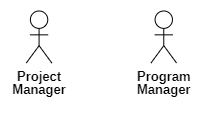
\includegraphics[width=0.3\columnwidth]{usecase/attori} 
    \caption{Attori}
\end{figure}
Gli attori che possiamo trovare all'interno dei casi d'uso rappresentano due risorse aziendali:
\subsubsection*{Project Manager}
Conosciuto come il "Responsabile di Progetto", si occupa dell'avvio, pianificazione ,esecuzione e controllo di un singolo progetto, seguendo tecniche di project management.\\
Le sue principali responsabilità sono:
\begin{itemize}
\item assicurarsi che i progetti siano allineati con gli obiettivi aziendali;
\item coordinare le risorse umane, assicurandosi che vengano utilizzate in modo efficiente;
\item stabilisce milestone, scadenze e obiettivi, monitorando lo stato di avanzamento dei progetti;
\item comunica con stakeholder, team di progetto e altre parti interessate.
\end{itemize}
\subsubsection*{Program Manager}
È un ruolo di gestione all'interno di un'organizzazione, ed è responsabile della pianificazione complessiva e del controllo di più progetti che compongono il suo programma. Collabora strettamente col Project Manager ed i loro compiti spesso si sovrappongono ma differiscono di portata, in quanto il Program Manager supervisiona gruppi di progetti gestiti singolarmente dai Project Manager.

\section{Casi d'uso}

\subsection{Scenario Anagrafiche}
\begin{figure}[H] 
    \centering 
    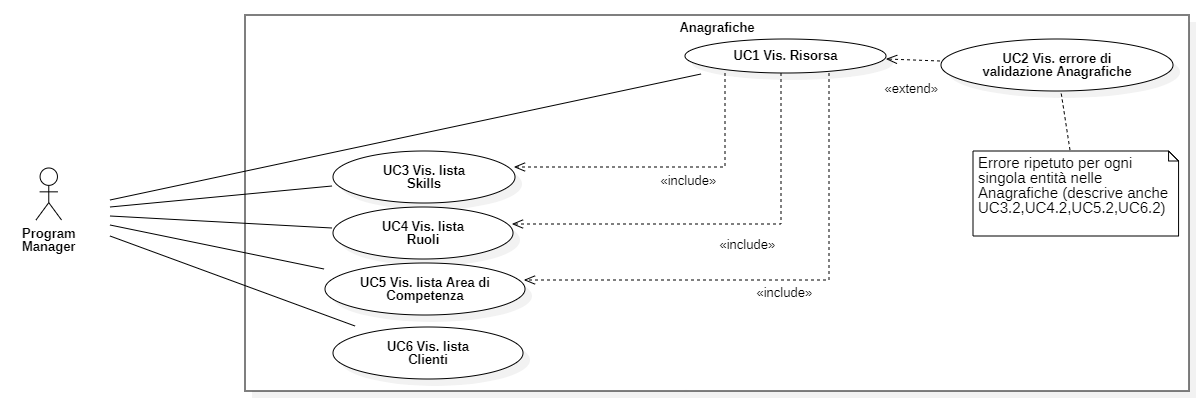
\includegraphics[width=1.1\columnwidth]{usecase/anagrafiche-general} 
    \caption{Casi d'Uso del scenario Anagrafiche}
\end{figure}

\subsubsection*{UC1 - Vis. Risorsa}

\begin{figure}[H] 
    \centering 
    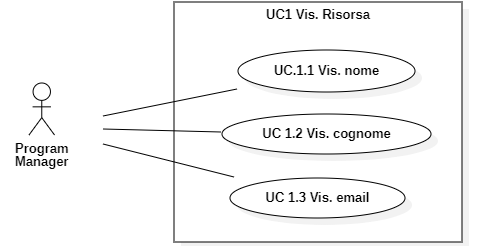
\includegraphics[width=0.6\columnwidth]{usecase/UC1} 
    \caption{Caso d'Uso 1 espanso}
\end{figure}

\begin{itemize}[label=$\circ$]
\item \textbf{Attore:} Program Manager;
\item \textbf{Descrizione:} il Program Manager può visualizzare una Risorsa;
\item \textbf{Precondizioni:} il richiedente è un Program Manager;
\item \textbf{Postcondizioni:} la Risorsa selezionata è visualizzabile dal Program Manager;
\item \textbf{Estensioni:} UC2;
\item \textbf{Inclusioni:} UC3, UC4, UC5.
\end{itemize}

\subsubsection*{UC1.1 - Vis. nome}
\begin{itemize}[label=$\circ$]
\item \textbf{Attore:} Program Manager;
\item \textbf{Descrizione:} il Program Manager può visualizzare il nome di una Risorsa;
\item \textbf{Precondizioni:} la Risorsa è visualizzabile dal Program Manager;
\item \textbf{Postcondizioni:} il Program Manager può visualizzare il nome della Risorsa selezionata;
\item \textbf{Estensioni:} il caso d'uso non ha estensioni;
\item \textbf{Inclusioni:} il caso d'uso non ha inclusioni.
\end{itemize}

\subsubsection*{UC1.2 - Vis. cognome}
\begin{itemize}[label=$\circ$]
\item \textbf{Attore:} Program Manager;
\item \textbf{Descrizione:} il Program Manager può visualizzare il cognome di una Risorsa;
\item \textbf{Precondizioni:}  la Risorsa è visualizzabile dal Program Manager;
\item \textbf{Postcondizioni:} il Program Manager può visualizzare il cognome della Risorsa selezionata;
\item \textbf{Estensioni:} il caso d'uso non ha estensioni;
\item \textbf{Inclusioni:} il caso d'uso non ha inclusioni.
\end{itemize}

\subsubsection*{UC1.3 - Vis. email}
\begin{itemize}[label=$\circ$]
\item \textbf{Attore:} Program Manager;
\item \textbf{Descrizione:} il Program Manager può visualizzare l'email di una Risorsa;
\item \textbf{Precondizioni:}  la Risorsa è visualizzabile dal Program Manager;
\item \textbf{Postcondizioni:} il Program Manager può visualizzare l'email della Risorsa selezionata;
\item \textbf{Estensioni:} il caso d'uso non ha estensioni;
\item \textbf{Inclusioni:} il caso d'uso non ha inclusioni.
\end{itemize}

\subsubsection*{UC2 - Vis. errore di validazione Anagrafiche}
\begin{itemize}[label=$\circ$]
\item \textbf{Attore:} Program Manager;
\item \textbf{Descrizione:} questo caso d'uso descrive anche UC3.2,UC4.2,UC5.2,UC6.2. Viene visualizzato un messaggio di errore in caso vengano eseguite funzionalità con dati non validi. Esso rappresenta errori di validazione nella richiesta fornita dall'utilizzatore;
\item \textbf{Precondizioni:} il Program Manager sta effettuando operazioni con dati non validi;
\item \textbf{Postcondizioni:} l'esecuzione della funzionalità è interrotta e viene visualizzato il messaggio di errore;
\item \textbf{Estensioni:} il caso d'uso non ha estensioni;
\item \textbf{Inclusioni:} il caso d'uso non ha inclusioni.
\end{itemize}

\subsubsection*{UC3 - Vis. lista Skill}
\begin{figure}[H] 
    \centering 
    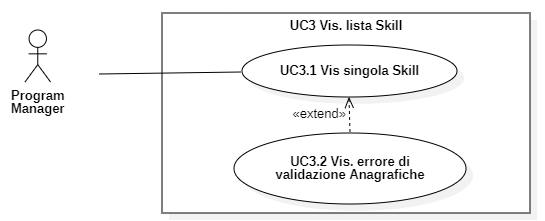
\includegraphics[width=0.6\columnwidth]{usecase/UC3} 
    \caption{Caso d'Uso 3 espanso}
\end{figure}
\begin{itemize}[label=$\circ$]
\item \textbf{Attore:} Program Manager;
\item \textbf{Descrizione:} il Program Manager può visualizzare la lista delle Skill;
\item \textbf{Precondizioni:} il richiedente è un Program Manager;
\item \textbf{Postcondizioni:} la lista delle Skill è visualizzabile dal Program Manager;
\item \textbf{Estensioni:} il caso d'uso non ha estensioni;
\item \textbf{Inclusioni:} il caso d'uso non ha inclusioni.
\end{itemize}

\subsubsection*{UC3.1 - Vis. singola Skill}
\begin{figure}[H] 
    \centering 
    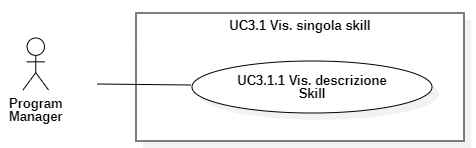
\includegraphics[width=0.6\columnwidth]{usecase/UC3.1} 
    \caption{Caso d'Uso 3.1 espanso}
\end{figure}
\begin{itemize}[label=$\circ$]
\item \textbf{Attore:} Program Manager;
\item \textbf{Descrizione:} il Program Manager può visualizzare una Skill;
\item \textbf{Precondizioni:} il richiedente è un Program Manager;
\item \textbf{Postcondizioni:} la Skill selezionata è visualizzabile dal Program Manager;
\item \textbf{Estensioni:} UC3.2;
\item \textbf{Inclusioni:} il caso d'uso non ha inclusioni.
\end{itemize}

\subsubsection*{UC3.1.1 - Vis. descrizione Skill}
\begin{itemize}[label=$\circ$]
\item \textbf{Attore:} Program Manager;
\item \textbf{Descrizione:} il Program Manager può visualizzare la descrizione di una Skill;
\item \textbf{Precondizioni:} la Skill è visualizzabile dal Program Manager;
\item \textbf{Postcondizioni:} il Program Manager può visualizzare la descrizione della Skill selezionata;
\item \textbf{Estensioni:} il caso d'uso non ha estensioni;
\item \textbf{Inclusioni:} il caso d'uso non ha inclusioni.
\end{itemize}

\subsubsection*{UC4 - Vis. lista Ruoli}
\begin{figure}[H] 
    \centering 
    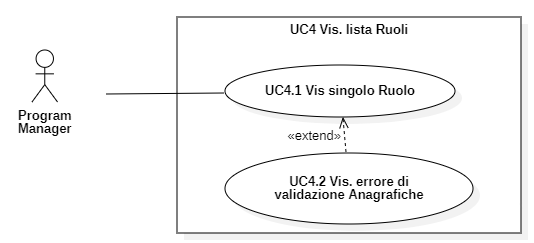
\includegraphics[width=0.6\columnwidth]{usecase/UC4} 
    \caption{Caso d'Uso 4 espanso}
\end{figure}
\begin{itemize}[label=$\circ$]
\item \textbf{Attore:} Program Manager;
\item \textbf{Descrizione:} il Program Manager può visualizzare la lista dei Ruoli;
\item \textbf{Precondizioni:} il richiedente è un Program Manager;
\item \textbf{Postcondizioni:} la lista dei Ruoli è visualizzabile dal Program Manager;
\item \textbf{Estensioni:} il caso d'uso non ha estensioni;
\item \textbf{Inclusioni:} il caso d'uso non ha inclusioni.
\end{itemize}

\subsubsection*{UC4.1 - Vis. singolo Ruolo}
\begin{figure}[H] 
    \centering 
    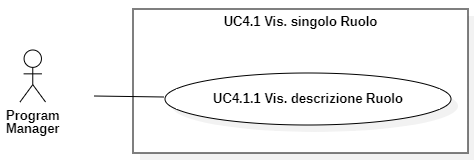
\includegraphics[width=0.6\columnwidth]{usecase/UC4.1} 
    \caption{Caso d'Uso 4.1 espanso}
\end{figure}
\begin{itemize}[label=$\circ$]
\item \textbf{Attore:} Program Manager;
\item \textbf{Descrizione:} il Program Manager può visualizzare un Ruolo;
\item \textbf{Precondizioni:} il richiedente è un Program Manager;
\item \textbf{Postcondizioni:} il Ruolo selezionato è visualizzabile dal Program Manager;
\item \textbf{Estensioni:}  UC4.2;
\item \textbf{Inclusioni:} il caso d'uso non ha inclusioni.
\end{itemize}

\subsubsection*{UC4.1.1 - Vis. descrizione Ruolo}
\begin{itemize}[label=$\circ$]
\item \textbf{Attore:} Program Manager;
\item \textbf{Descrizione:} il Program Manager può visualizzare la descrizione di un Ruolo;
\item \textbf{Precondizioni:}  il Ruolo è visualizzabile dal Program Manager;
\item \textbf{Postcondizioni:} il Program Manager può visualizzare la descrizione del Ruolo selezionato;
\item \textbf{Estensioni:} il caso d'uso non ha estensioni;
\item \textbf{Inclusioni:} il caso d'uso non ha inclusioni.
\end{itemize}

\subsubsection*{UC5 - Vis. lista Area di Competenza}
\begin{figure}[H] 
    \centering 
    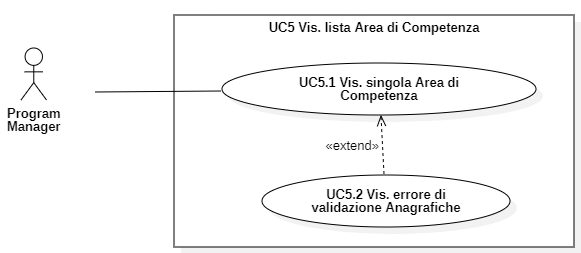
\includegraphics[width=0.6\columnwidth]{usecase/UC5} 
    \caption{Caso d'Uso 5 espanso}
\end{figure}
\begin{itemize}[label=$\circ$]
\item \textbf{Attore:} Program Manager;
\item \textbf{Descrizione:} il Program Manager può visualizzare la lista delle Aree di Competenza;
\item \textbf{Precondizioni:} il richiedente è un Program Manager;
\item \textbf{Postcondizioni:} la lista delle Aree di Competenza è visualizzabile dal Program Manager;
\item \textbf{Estensioni:} il caso d'uso non ha estensioni;
\item \textbf{Inclusioni:} il caso d'uso non ha inclusioni.
\end{itemize}

\subsubsection*{UC5.1 - Vis. singola Area di Competenza}
\begin{figure}[H] 
    \centering 
    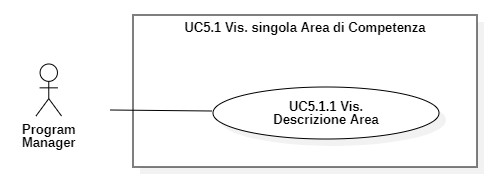
\includegraphics[width=0.6\columnwidth]{usecase/UC5.1} 
    \caption{Caso d'Uso 5.1 espanso}
\end{figure}
\begin{itemize}[label=$\circ$]
\item \textbf{Attore:} Program Manager;
\item \textbf{Descrizione:} il Program Manager può visualizzare un'Area di Competenza;
\item \textbf{Precondizioni:} il richiedente è un Program Manager;
\item \textbf{Postcondizioni:} l'Area di Competenza selezionata è visualizzabile dal Program Manager;
\item \textbf{Estensioni:}  UC5.2;
\item \textbf{Inclusioni:} il caso d'uso non ha inclusioni.
\end{itemize}

\subsubsection*{UC5.1.1 - Vis. descrizione Area}
\begin{itemize}[label=$\circ$]
\item \textbf{Attore:} Program Manager;
\item \textbf{Descrizione:} il Program Manager può visualizzare la descrizione di un'Area di Competenza;
\item \textbf{Precondizioni:}  l'Area è visualizzabile dal Program Manager;
\item \textbf{Postcondizioni:} il Program Manager può visualizzare la descrizione dell'Area di Competenza selezionata;
\item \textbf{Estensioni:} non ci sono estensioni;
\item \textbf{Inclusioni:} non ci sono inclusioni.
\end{itemize}

\subsubsection*{UC6 - Vis. lista Clienti}
\begin{figure}[H] 
    \centering 
    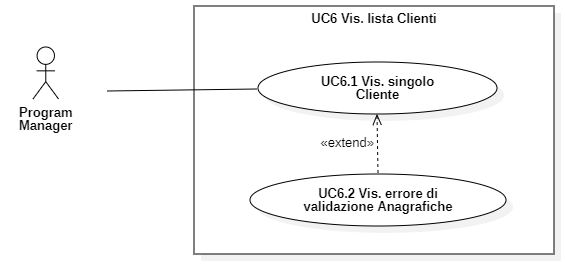
\includegraphics[width=0.6\columnwidth]{usecase/UC6} 
    \caption{Caso d'Uso 6 espanso}
\end{figure}
\begin{itemize}[label=$\circ$]
\item \textbf{Attore:} Program Manager;
\item \textbf{Descrizione:} il Program Manager può visualizzare la lista dei Clienti;
\item \textbf{Precondizioni:} il richiedente è un Program Manager;
\item \textbf{Postcondizioni:} la lista dei Clienti è visualizzabile dal Program Manager;
\item \textbf{Estensioni:} il caso d'uso non ha estensioni;
\item \textbf{Inclusioni:} il caso d'uso non ha inclusioni.
\end{itemize}

\subsubsection*{UC6.1 - Vis. singolo Cliente}
\begin{figure}[H] 
    \centering 
    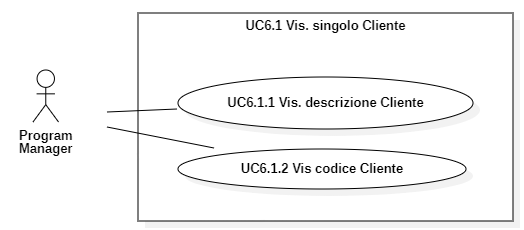
\includegraphics[width=0.6\columnwidth]{usecase/UC6.1} 
    \caption{Caso d'Uso 6.1 espanso}
\end{figure}
\begin{itemize}[label=$\circ$]
\item \textbf{Attore:} Program Manager;
\item \textbf{Descrizione:} il Program Manager può visualizzare un Cliente;
\item \textbf{Precondizioni:} il richiedente è un Program Manager;
\item \textbf{Postcondizioni:} il Cliente selezionato è visualizzabile dal Program Manager;
\item \textbf{Estensioni:} UC6.2;
\item \textbf{Inclusioni:} non ci sono inclusioni.
\end{itemize}

\subsubsection*{UC6.1.1 - Vis. descrizione Cliente}
\begin{itemize}[label=$\circ$]
\item \textbf{Attore:} Program Manager;
\item \textbf{Descrizione:} il Program Manager può visualizzare la descrizione di Cliente;
\item \textbf{Precondizioni:}  il Cliente è visualizzabile dal Program Manager;
\item \textbf{Postcondizioni:} il Program Manager può visualizzare la descrizione del Cliente selezionato;
\item \textbf{Estensioni:} il caso d'uso non ha estensioni;
\item \textbf{Inclusioni:} il caso d'uso non ha inclusioni.
\end{itemize}

\subsubsection*{UC6.1.2 - Vis. codice Cliente}
\begin{itemize}[label=$\circ$]
\item \textbf{Attore:} Program Manager;
\item \textbf{Descrizione:} il Program Manager può visualizzare il codice del Cliente;
\item \textbf{Precondizioni:} il Cliente è visualizzabile dal Program Manager;
\item \textbf{Postcondizioni:} il Program Manager può visualizzare il codice del Cliente selezionato;
\item \textbf{Estensioni:} il caso d'uso non ha estensioni;
\item \textbf{Inclusioni:} il caso d'uso non ha inclusioni.
\end{itemize}


\subsection{Scenario Richieste}
\begin{figure}[H] 
    \centering 
    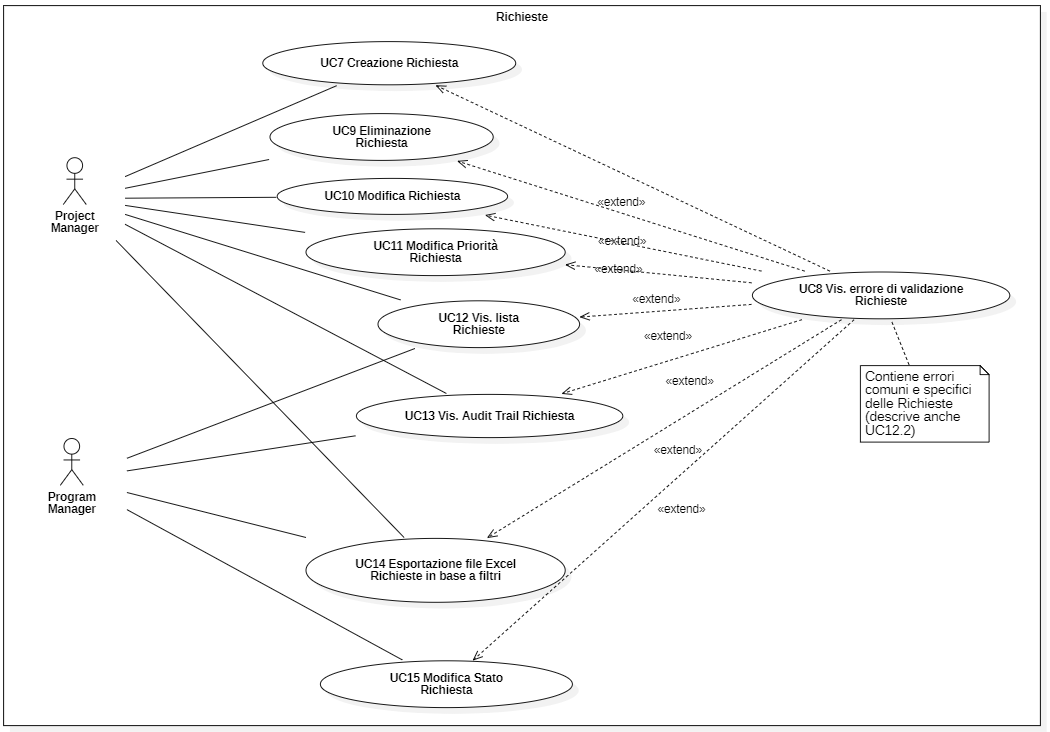
\includegraphics[width=1.1\columnwidth]{usecase/richieste-general} 
    \caption{Casi d'Uso del scenario Richieste}
\end{figure}

\subsubsection*{UC7 - Creazione Richiesta}
\begin{itemize}[label=$\circ$]
\item \textbf{Attore:} Project Manager;
\item \textbf{Descrizione:} il Project Manager può creare una nuova Richiesta;
\item \textbf{Precondizioni:} il richiedente è un Project Manager;
\item \textbf{Postcondizioni:} la Richiesta è stata creata dal Project Manager con successo;
\item \textbf{Estensioni:} UC8;
\item \textbf{Inclusioni:} il caso d'uso non ha inclusioni.
\end{itemize}

\subsubsection*{UC8 - Vis. errore di validazione Richieste}
\begin{itemize}[label=$\circ$]
\item \textbf{Attore:} Project Manager e Program Manager;
\item \textbf{Descrizione:}  questo caso d'uso descrive anche UC12.2. Viene visualizzato un messaggio di errore in caso vengano eseguite funzionalità con dati non validi. Esso rappresenta i seguenti errori comuni all'interno delle Richieste: dati non validi, filtri non valorizzati, entità associate non valide, risultati nulli o non valorizzati;
\item \textbf{Precondizioni:} il Program Manger o il Project Manager stanno effettuando operazioni con dati non validi;
\item \textbf{Postcondizioni:} l'esecuzione della funzionalità è interrotta e viene visualizzato il messaggio di errore;
\item \textbf{Estensioni:} il caso d'uso non ha estensioni;
\item \textbf{Inclusioni:} il caso d'uso non ha inclusioni.
\end{itemize}

\subsubsection*{UC9 - Eliminazione Richiesta}
\begin{itemize}[label=$\circ$]
\item \textbf{Attore:} Project Manager;
\item \textbf{Descrizione:} il Project Manager può eliminare una Richiesta esistente;
\item \textbf{Precondizioni:} il richiedente è un Project Manager;
\item \textbf{Postcondizioni:} la Richiesta è stata eliminata dal Project Manager con successo;
\item \textbf{Estensioni:} UC8;
\item \textbf{Inclusioni:} il caso d'uso non ha inclusioni.
\end{itemize}

\subsubsection*{UC10 - Modifica Richiesta}
\begin{itemize}[label=$\circ$]
\item \textbf{Attore:} Project Manager;
\item \textbf{Descrizione:} il Project Manager può modificare una Richiesta esistente nella sua totalità sovrascrivendola;
\item \textbf{Precondizioni:} il richiedente è un Project Manager;
\item \textbf{Postcondizioni:} la Richiesta selezionata è stata modificata con successo;
\item \textbf{Estensioni:} UC8;
\item \textbf{Inclusioni:} il caso d'uso non ha inclusioni.
\end{itemize}

\subsubsection*{UC11 - Modifica Priorità Richiesta}
\begin{itemize}[label=$\circ$]
\item \textbf{Attore:} Project Manager;
\item \textbf{Descrizione:} il Project Manager può modificare l'attributo Priorità di una Richiesta esistente inserendo un valore tra: Alta, Media o Bassa;
\item \textbf{Precondizioni:} il richiedente è un Project Manager;
\item \textbf{Postcondizioni:} la Richiesta è stata modificata con successo solo nel campo Priorità dal Project Manager;
\item \textbf{Estensioni:} UC8;
\item \textbf{Inclusioni:} il caso d'uso non ha inclusioni.
\end{itemize}

\subsubsection*{UC12 - Vis. lista Richieste}

\begin{figure}[H] 
    \centering 
    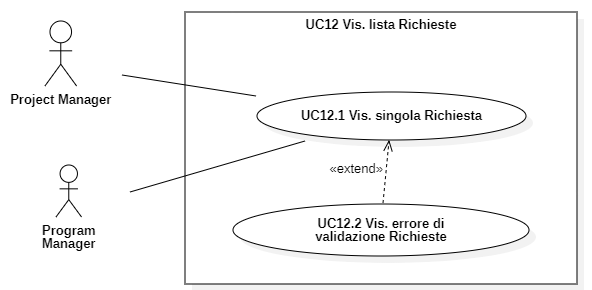
\includegraphics[width=0.6\columnwidth]{usecase/UC12} 
    \caption{Caso d'Uso 12 espanso}
\end{figure}

\begin{itemize}[label=$\circ$]
\item \textbf{Attore:} Project Manager e Program Manager;
\item \textbf{Descrizione:} il Project Manager e il Program Manager possono visualizzare una lista di Richieste dopo aver inserito filtri e/o una parola nella ricerca rapida e aver selezionato se i filtri applicati devono essere congiunti o disgiunti;
\item \textbf{Precondizioni:} il richiedente è un Project Manager o un Program Manager;
\item \textbf{Postcondizioni:} la lista delle Richieste è visualizzabile dal Project Manager e dal Program Manager;
\item \textbf{Estensioni:} UC8;
\item \textbf{Inclusioni:} il caso d'uso non ha inclusioni.
\end{itemize}

\subsubsection*{UC12.1 - Vis. singola Richiesta}

\begin{figure}[H] 
    \centering 
    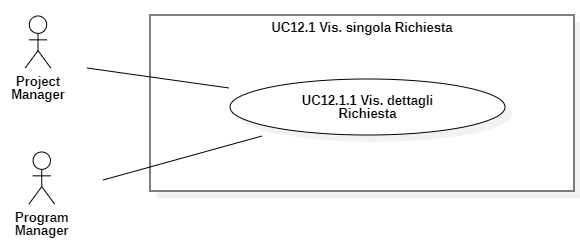
\includegraphics[width=0.6\columnwidth]{usecase/UC12.1} 
    \caption{Caso d'Uso 12.1 espanso}
\end{figure}

\begin{itemize}[label=$\circ$]
\item \textbf{Attore:} Project Manager e Program Manager;
\item \textbf{Descrizione:} il Project Manager e il Program Manager possono visualizzare la Richiesta selezionata;
\item \textbf{Precondizioni:} la lista delle Richieste è visualizzabile;
\item \textbf{Postcondizioni:} la Richiesta selezionata è visualizzabile dal Program Manager e dal Project Manager;
\item \textbf{Estensioni:} UC12.2;
\item \textbf{Inclusioni:} il caso d'uso non ha inclusioni.
\end{itemize}

\subsubsection*{UC12.1.1 - Vis. dettagli Richiesta}

\begin{figure}[H] 
    \centering 
    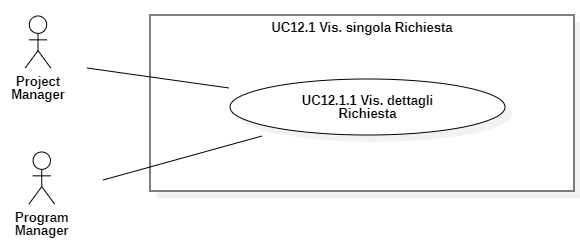
\includegraphics[width=0.6\columnwidth]{usecase/UC12.1} 
    \caption{Caso d'Uso 12.1 espanso}
\end{figure}

\begin{itemize}[label=$\circ$]
\item \textbf{Attore:} Project Manager e Program Manager;
\item \textbf{Descrizione:} il Project Manager e il Program Manager possono visualizzare la Richiesta selezionata;
\item \textbf{Precondizioni:} la Richiesta singola è visualizzabile;
\item \textbf{Postcondizioni:} il Project Manager e il Program Manager possono visualizzare i campi di una Richiesta selezionata;
\item \textbf{Estensioni:} il caso d'uso non ha esclusioni;
\item \textbf{Inclusioni:} il caso d'uso non ha inclusioni.
\end{itemize}

\subsubsection*{UC13 - Vis. audit trail Richiesta}

\begin{figure}[H] 
    \centering 
    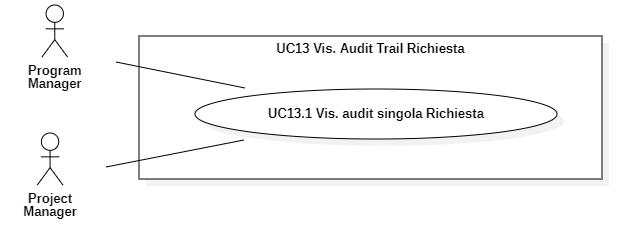
\includegraphics[width=0.6\columnwidth]{usecase/UC13} 
    \caption{Caso d'Uso 13 espanso}
\end{figure}

\begin{itemize}[label=$\circ$]
\item \textbf{Attore:} Project Manager e Program Manager;
\item \textbf{Descrizione:} il Project Manager e il Program Manager possono visualizzare l'audit trail di una Richiesta selezionata.;
\item \textbf{Precondizioni:} il richiedente è un Project Manager o un Program Manager;
\item \textbf{Postcondizioni:} la traccia di audit della Richiesta selezionata è visualizzabile dal Project Manager e dal Program Manager;
\item \textbf{Estensioni:} UC8;
\item \textbf{Inclusioni:} il caso d'uso non ha inclusioni.
\end{itemize}

\subsubsection*{UC13.1 - Vis. audit singola Richiesta}

\begin{figure}[H] 
    \centering 
    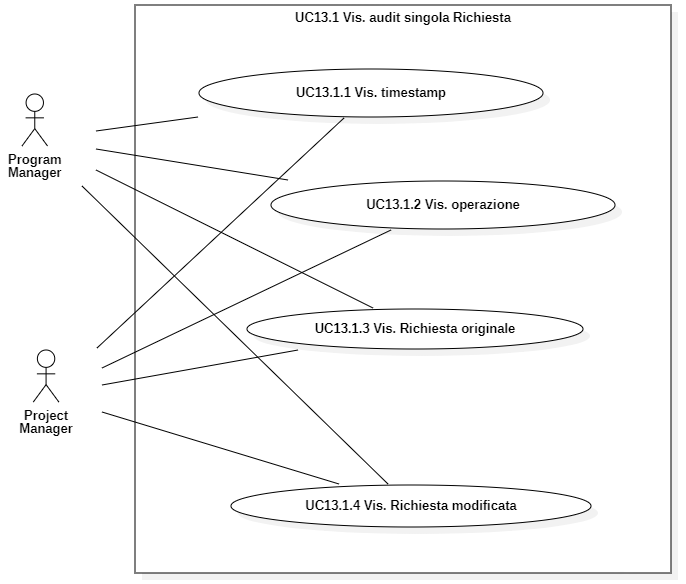
\includegraphics[width=0.8\columnwidth]{usecase/UC13.1} 
    \caption{Caso d'Uso 13.1 espanso}
\end{figure}

\begin{itemize}[label=$\circ$]
\item \textbf{Attore:} Project Manager e Program Manager;
\item \textbf{Descrizione:} il Project Manager e il Program Manager possono visualizzare l'audit di una singola Richiesta;
\item \textbf{Precondizioni:} l'audit trail è visualizzabile;
\item \textbf{Postcondizioni:} l'audit di una singola Richiesta è visualizzabile;
\item \textbf{Estensioni:} il caso d'uso non ha estensioni;
\item \textbf{Inclusioni:} il caso d'uso non ha inclusioni.
\end{itemize}

\subsubsection*{UC13.1.1 - Vis. timestamp}
\begin{itemize}[label=$\circ$]
\item \textbf{Attore:} Project Manager e Program Manager;
\item \textbf{Descrizione:} il Project Manager e il Program Manager possono visualizzare il timestamp di una singola audit di una Richiesta;
\item \textbf{Precondizioni:} la singola audit di una Richiesta è visualizzabile;
\item \textbf{Postcondizioni:} il timestamp della singola audit è visualizzabile;
\item \textbf{Estensioni:} il caso d'uso non ha estensioni;
\item \textbf{Inclusioni:} il caso d'uso non ha inclusioni.
\end{itemize}

\subsubsection*{UC13.1.2 - Vis. operazione}
\begin{itemize}[label=$\circ$]
\item \textbf{Attore:} Project Manager e Program Manager;
\item \textbf{Descrizione:} il Project Manager e il Program Manager possono visualizzare l'operazione di una singola audit di una Richiesta;
\item \textbf{Precondizioni:} la singola audit di una Richiesta è visualizzabile;
\item \textbf{Postcondizioni:} l'operazione della singola audit è visualizzabile;
\item \textbf{Estensioni:} il caso d'uso non ha estensioni;
\item \textbf{Inclusioni:} il caso d'uso non ha inclusioni.
\end{itemize}

\subsubsection*{UC13.1.3 - Vis. Richiesta originale}
\begin{itemize}[label=$\circ$]
\item \textbf{Attore:} Project Manager e Program Manager;
\item \textbf{Descrizione:} il Project Manager e il Program Manager possono visualizzare la singola audit di una Richiesta prima che l'operazione venga eseguita;
\item \textbf{Precondizioni:} la singola audit di una Richiesta è visualizzabile;
\item \textbf{Postcondizioni:} la Richiesta originale della singola audit è visualizzabile;
\item \textbf{Estensioni:} il caso d'uso non ha estensioni;
\item \textbf{Inclusioni:} il caso d'uso non ha inclusioni.
\end{itemize}

\subsubsection*{UC13.1.4 - Vis. Richiesta modificata}
\begin{itemize}[label=$\circ$]
\item \textbf{Attore:} Project Manager e Program Manager;
\item \textbf{Descrizione:} il Project Manager e il Program Manager possono visualizzare la singola audit di una Richiesta dopo che l'operazione è stata eseguita;
\item \textbf{Precondizioni:} la singola audit di una Richiesta è visualizzabile;
\item \textbf{Postcondizioni:} la Richiesta modificata della singola audit è visualizzabile;
\item \textbf{Estensioni:} il caso d'uso non ha estensioni;
\item \textbf{Inclusioni:} il caso d'uso non ha inclusioni.
\end{itemize}

\subsubsection*{UC14 - Esportazione file Excel Richieste in base a filtri}
\begin{itemize}[label=$\circ$]
\item \textbf{Attore:} Project Manager e Program Manager;
\item \textbf{Descrizione:} il Project Manager e il Program Manager possono esportare in un file Excel scaricabile un report delle Richieste in base a dei filtri inseriti;
\item \textbf{Precondizioni:} il richiedente è un Project Manager o un Program Manager;
\item \textbf{Postcondizioni:} il report Excel è stato generato correttamente ed è possibile scaricarlo;
\item \textbf{Estensioni:} UC8;
\item \textbf{Inclusioni:} il caso d'uso non ha inclusioni.
\end{itemize}

\subsubsection*{UC15 - Modifica Stato Richiesta}
\begin{itemize}[label=$\circ$]
\item \textbf{Attore:} Program Manager;
\item \textbf{Descrizione:} il Program Manager può cambiare lo stato di una Richiesta esistente impostandolo in uno dei seguenti valori: Evasa, Non Evasa, Aperta, In corso, Chiusa;
\item \textbf{Precondizioni:} il richiedente è un Program Manager;
\item \textbf{Postcondizioni:} solo lo stato della Richiesta è stato modificato con successo;
\item \textbf{Estensioni:} UC8;
\item \textbf{Inclusioni:} il caso d'uso non ha inclusioni.
\end{itemize}



\subsection{Scenario Pianificazioni}
\begin{figure}[H] 
    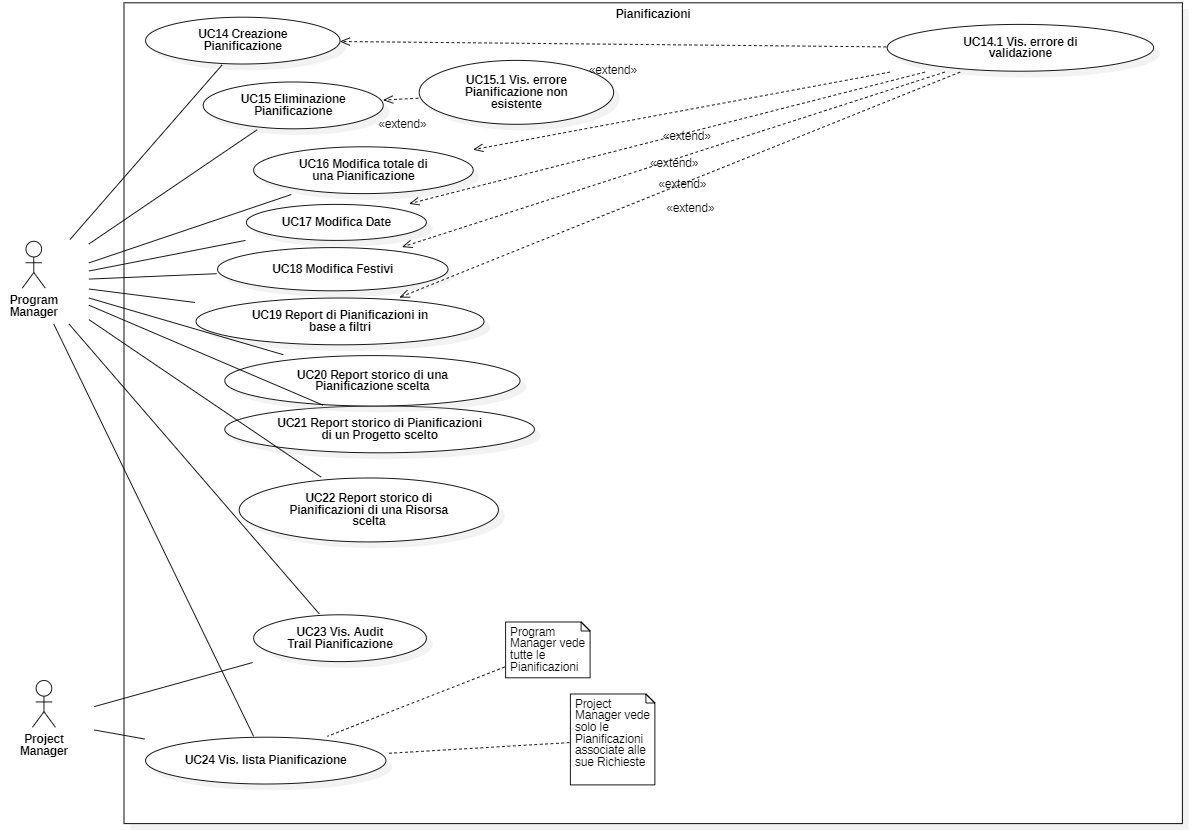
\includegraphics[width=1.00\linewidth]{usecase/pianificazioni-general} 
    \caption{Casi d'Uso del scenario Pianificazioni}
\end{figure}

\subsubsection*{UC16 - Creazione Pianificazione}
\begin{itemize}[label=$\circ$]
\item \textbf{Attore:} Program Manager;
\item \textbf{Descrizione:} il Program Manager può creare una Pianificazione per Figura richiesta da una Richiesta;
\item \textbf{Precondizioni:} il richiedente è un Program Manager;
\item \textbf{Postcondizioni:} la Pianificazione è stata creata dal Program Manager con successo;
\item \textbf{Estensioni:} UC17;
\item \textbf{Inclusioni:} il caso d'uso non ha inclusioni.
\end{itemize}

\subsubsection*{UC17 - Vis. errore di validazione Pianificazioni}
\begin{itemize}[label=$\circ$]
\item \textbf{Attore:} Project Manager e Program Manager;
\item \textbf{Descrizione:} questo caso d'uso descrive anche UC26.2. Viene visualizzato un messaggio di errore in caso vengano eseguite funzionalità con dati non validi. Esso rappresenta i seguenti errori comuni all'interno delle Pianificazioni: dati non validi, filtri non valorizzati, entità associate non valide, risultati nulli o non valorizzati;
\item \textbf{Precondizioni:} il Program Manager o il Project Manager stanno effettuando operazioni con dati non validi;
\item \textbf{Postcondizioni:} l'esecuzione della funzionalità è interrotta e viene visualizzato il messaggio di errore;
\item \textbf{Estensioni:} il caso d'uso non ha estensioni;
\item \textbf{Inclusioni:} il caso d'uso non ha inclusioni.
\end{itemize}

\subsubsection*{UC18 - Eliminazione Pianificazione}
\begin{itemize}[label=$\circ$]
\item \textbf{Attore:} Program Manager;
\item \textbf{Descrizione:} il Program Manager può eliminare una Pianificazione esistente;
\item \textbf{Precondizioni:} il richiedente è il Program Manager;
\item \textbf{Postcondizioni:} la Pianificazione è stata eliminata dal Program Manager con successo;
\item \textbf{Estensioni:} UC17;
\item \textbf{Inclusioni:} il caso d'uso non ha inclusioni.
\end{itemize}

\subsubsection*{UC19 - Modifica Pianificazione}
\begin{itemize}[label=$\circ$]
\item \textbf{Attore:} Program Manager;
\item \textbf{Descrizione:} il Program Manager può modificare una Pianificazione esistente nella sua totalità sovrascrivendola;
\item \textbf{Precondizioni:} il richiedente è un Program Manager;
\item \textbf{Postcondizioni:} la Pianificazione selezionata è stata modificata con successo;
\item \textbf{Estensioni:} UC17;
\item \textbf{Inclusioni:} il caso d'uso non ha inclusioni.
\end{itemize}

\subsubsection*{UC20 - Modifica Date}
\begin{itemize}[label=$\circ$]
\item \textbf{Attore:} Program Manager;
\item \textbf{Descrizione:} il Program Manager può modificare le date di inizio e/o di fine di una Pianificazione;
\item \textbf{Precondizioni:} il richiedente è un Program Manager;
\item \textbf{Postcondizioni:} la Pianificazione è stata modificata con successo solo nel campo Data inizio e/o Data fine dal Program Manager;
\item \textbf{Estensioni:} UC17;
\item \textbf{Inclusioni:} il caso d'uso non ha inclusioni.
\end{itemize}

\subsubsection*{UC21 - Modifica Festivi}
\begin{itemize}[label=$\circ$]
\item \textbf{Attore:} Program Manager;
\item \textbf{Descrizione:} il Porgram Manager può modificare il campo Festivi di una Pianificazione. Se posto a vero il lavoratore potrà lavorare anche nei giorni festivi;
\item \textbf{Precondizioni:} il richiedente è un Program Manager;
\item \textbf{Postcondizioni:}  la Pianificazione è stata modificata con successo solo nel campo Festivi dal Program Manager;
\item \textbf{Estensioni:} UC17;
\item \textbf{Inclusioni:} il caso d'uso non ha inclusioni.
\end{itemize}

\subsubsection*{UC22 - Esportazione file Excel di Pianificazioni in base a filtri}
\begin{itemize}[label=$\circ$]
\item \textbf{Attore:} Program Manager;
\item \textbf{Descrizione:} : il Program Manager può esportare in un
file Excel scaricabile un report delle Pianificazioni in base a dei filtri inseriti;
\item \textbf{Precondizioni:} : il richiedente è un Program Manager;
\item \textbf{Postcondizioni:} il report Excel è stato generato correttamente ed è possibile
scaricarlo;
\item \textbf{Estensioni:} UC17;
\item \textbf{Inclusioni:} il caso d'uso non ha inclusioni.
\end{itemize}

\subsubsection*{UC23 - Esportazione storico Excel di Pianificazioni di un Progetto}
\begin{itemize}[label=$\circ$]
\item \textbf{Attore:} Program Manager;
\item \textbf{Descrizione:} il Program Manager può esportare in un file Excel scaricabile uno storico di Pianificazioni associate ad un Progetto contenente tutte le risorse allocate e l’effettivo impiego di queste nelle attività;
\item \textbf{Precondizioni:} il richiedente è un Program Manager;
\item \textbf{Postcondizioni:} il report Excel è stato generato correttamente ed è possibile
scaricarlo;
\item \textbf{Estensioni:} UC17;
\item \textbf{Inclusioni:} il caso d'uso non ha inclusioni.
\end{itemize}

\subsubsection*{UC24 - Esportazione storico Excel di Pianificazioni di una Risorsa}
\begin{itemize}[label=$\circ$]
\item \textbf{Attore:} Program Manager;
\item \textbf{Descrizione:} il Program Manager può esportare in un file Excel scaricabile uno storico di Pianificazioni in cui c'è stata una determinata Risorsa;
\item \textbf{Precondizioni:} il richiedente è un Program Manager;
\item \textbf{Postcondizioni:} il report Excel è stato generato correttamente ed è possibile
scaricarlo;
\item \textbf{Estensioni:} UC17;
\item \textbf{Inclusioni:} il caso d'uso non ha inclusioni.
\end{itemize}

\subsubsection*{UC25 - Vis. Audit Trail Pianificazione}
\begin{figure}[H] 
    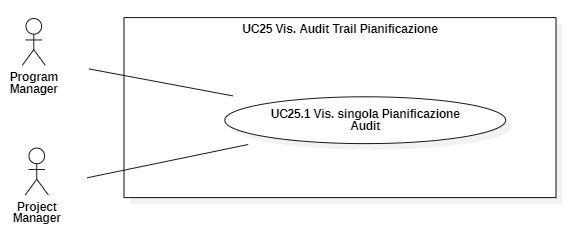
\includegraphics[width=0.65\linewidth]{usecase/UC25} 
    \caption{Caso d'Uso 25 espanso}
\end{figure}

\begin{itemize}[label=$\circ$]
\item \textbf{Attore:} Project Manager o Program Manager;
\item \textbf{Descrizione:} il Project Manager o il Program Manager possono visualizzare
l’audit trail di una Richiesta selezionata. Il Project Manager può vedere solo le tracce di audit delle Pianificazioni associate alle sue Richieste, mentre il Program Manager può vederle tutte;
\item \textbf{Precondizioni:} il richiedente è un Program Manager o un Project Manager;
\item \textbf{Postcondizioni:} la traccia di audit della Pianificazione selezionata è visualizzabile dal Project Manager o dal Program Manager;
\item \textbf{Estensioni:} UC17;
\item \textbf{Inclusioni:} il caso d'uso non ha inclusioni.
\end{itemize}


\subsubsection*{UC25.1 - Vis. singola Pianificazione Audit}
\begin{figure}[H] 
    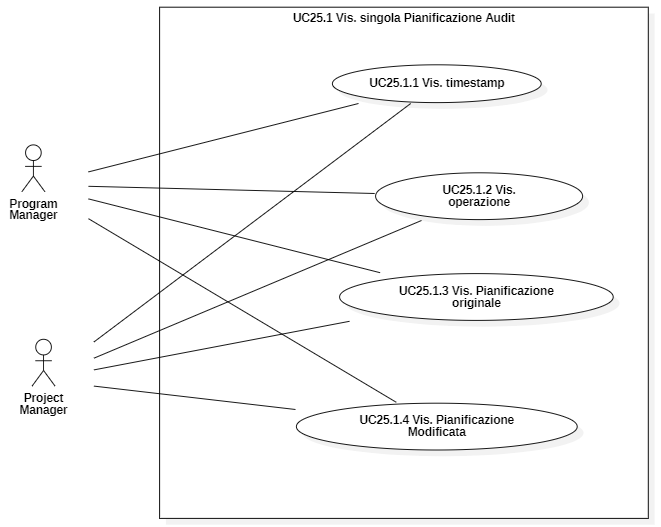
\includegraphics[width=0.75\linewidth]{usecase/UC25.1} 
    \caption{Caso d'Uso 25.1 espanso}
\end{figure}

\begin{itemize}[label=$\circ$]
\item \textbf{Attore:} Project Manager o Program Manager;
\item \textbf{Descrizione:} il Project Manager o il Program Manager può vedere l'audit di una singola Pianificazione. Il Project Manager può vedere solo le Pianificazioni associate alle sue Richieste, mentre il Program Manager può vederle tutte;
\item \textbf{Precondizioni:} l'audit trail è visualizzabile;
\item \textbf{Postcondizioni:} l'audit di una singola Pianificazione è visualizzabile;
\item \textbf{Estensioni:} il caso d'uso non ha estensioni;
\item \textbf{Inclusioni:} il caso d'uso non ha inclusioni.
\end{itemize}

\subsubsection*{UC25.1.1 - Vis. timestamp}

\begin{itemize}[label=$\circ$]
\item \textbf{Attore:} Project Manager o Program Manager;
\item \textbf{Descrizione:} il Project Manager e il Program Manager possono visualizzare il
timestamp di una singola audit di una Pianificazione;
\item \textbf{Precondizioni:} la singola audit di una Pianificazione è visualizzabile;
\item \textbf{Postcondizioni:} il timestamp della singola audit è visualizzabile;
\item \textbf{Estensioni:} il caso d'uso non ha estensioni;
\item \textbf{Inclusioni:} il caso d'uso non ha inclusioni.
\end{itemize}

\subsubsection*{UC25.1.2 - Vis. operazione}

\begin{itemize}[label=$\circ$]
\item \textbf{Attore:} Project Manager o Program Manager;
\item \textbf{Descrizione:} il Project Manager e il Program Manager possono visualizzare l'operazione di una singola audit di una Pianificazione;
\item \textbf{Precondizioni:} la singola audit di una Pianificazione è visualizzabile;
\item \textbf{Postcondizioni:} l’operazione della singola audit è visualizzabile;
\item \textbf{Estensioni:} il caso d'uso non ha estensioni;
\item \textbf{Inclusioni:} il caso d'uso non ha inclusioni.
\end{itemize}

\subsubsection*{UC25.1.3 - Vis. Pianificazione originale}

\begin{itemize}[label=$\circ$]
\item \textbf{Attore:} Project Manager o Program Manager;
\item \textbf{Descrizione:} il Project Manager o il Program Manager possono visualizzare la
singola audit di una Pianificazione prima che l’operazione venga eseguita;
\item \textbf{Precondizioni:}la singola audit di una Pianificazione è visualizzabile;
\item \textbf{Postcondizioni:} la Richiesta originale della singola audit è visualizzabile;
\item \textbf{Estensioni:} il caso d'uso non ha estensioni;
\item \textbf{Inclusioni:} il caso d'uso non ha inclusioni.
\end{itemize}

\subsubsection*{UC25.1.4 - Vis. Pianificazione modificata}

\begin{itemize}[label=$\circ$]
\item \textbf{Attore:} Project Manager o Program Manager;
\item \textbf{Descrizione:} il Project Manager o il Program Manager possono visualizzare la
singola audit di una Pianificazione dopo che l’operazione è stata eseguita;
\item \textbf{Precondizioni:} la singola audit di una Pianificazione è visualizzabile;
\item \textbf{Postcondizioni:} la Pianificazione modificata della singola audit è visualizzabile;
\item \textbf{Estensioni:} il caso d'uso non ha estensioni;
\item \textbf{Inclusioni:} il caso d'uso non ha inclusioni.
\end{itemize}

\subsubsection*{UC26 - Vis. lista Pianificazione}
\begin{figure}[H] 
    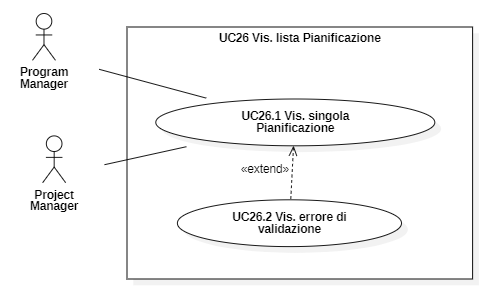
\includegraphics[width=0.65\linewidth]{usecase/UC26} 
    \caption{Caso d'Uso 26 espanso}
\end{figure}

\begin{itemize}[label=$\circ$]
\item \textbf{Attore:}  Project Manager o Program Manager;
\item \textbf{Descrizione:} il Project Manager o il Program Manager possono visualizzare
una lista di Richieste dopo aver inserito filtri e/o una parola nella ricerca rapida
e aver selezionato se i filtri applicati devono essere congiunti o disgiunti. Il Project Manager può vedere solo le Pianificazioni associate alle sue Richieste, mentre il Program Manager può vederle tutte;
\item \textbf{Precondizioni:} il richiedente è un Project Manager o un Program Manager;
\item \textbf{Postcondizioni:} la lista delle Richieste è visualizzabile dal Project Manager o dal Program Manager;
\item \textbf{Estensioni:} UC17;
\item \textbf{Inclusioni:} il caso d'uso non ha inclusioni.
\end{itemize}


\subsubsection*{UC26.1 - Vis. singola Pianificazione}
\begin{figure}[H] 
    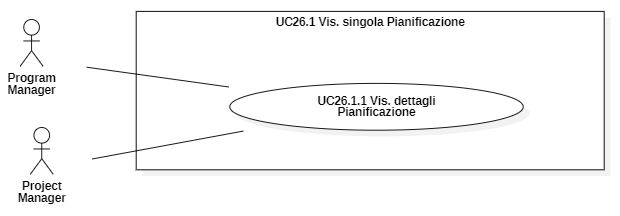
\includegraphics[width=0.75\linewidth]{usecase/UC26.1} 
    \caption{Caso d'Uso 26.1 espanso}
\end{figure}

\begin{itemize}[label=$\circ$]
\item \textbf{Attore:}  Project Manager o Program Manager;
\item \textbf{Descrizione:} il Project Manager o il Program Manager possono visualizzare la Pianificazione selezionata. Il Project Manager può vedere solo le Pianificazioni associate alle sue Richieste, mentre il Program Manager può vederle tutte;
\item \textbf{Precondizioni:} la lista delle Pianificazioni è visualizzabile;
\item \textbf{Postcondizioni:} la Pianificazione selezionata è visualizzabile dal Program Manager o dal Project Manager;
\item \textbf{Estensioni:} UC26.2;
\item \textbf{Inclusioni:} il caso d'uso non ha inclusioni.
\end{itemize}

\subsubsection*{UC26.1.1 - Vis. dettagli Pianificazione}
\begin{itemize}[label=$\circ$]
\item \textbf{Attore:}  Project Manager o Program Manager;
\item \textbf{Descrizione:} il Project Manager o il Program Manager possono visualizzare la
Pianificazione selezionata;
\item \textbf{Precondizioni:} la Pianificazione singola è visualizzabile;
\item \textbf{Postcondizioni:} il Project Manager e il Program Manager possono visualizzare
i campi di una Pianificazione selezionata;
\item \textbf{Estensioni:} il caso d'uso non ha estensioni;
\item \textbf{Inclusioni:} il caso d'uso non ha inclusioni.
\end{itemize}




\subsection{Scenario Milestone}
\begin{figure}[H] 
    \centering 
    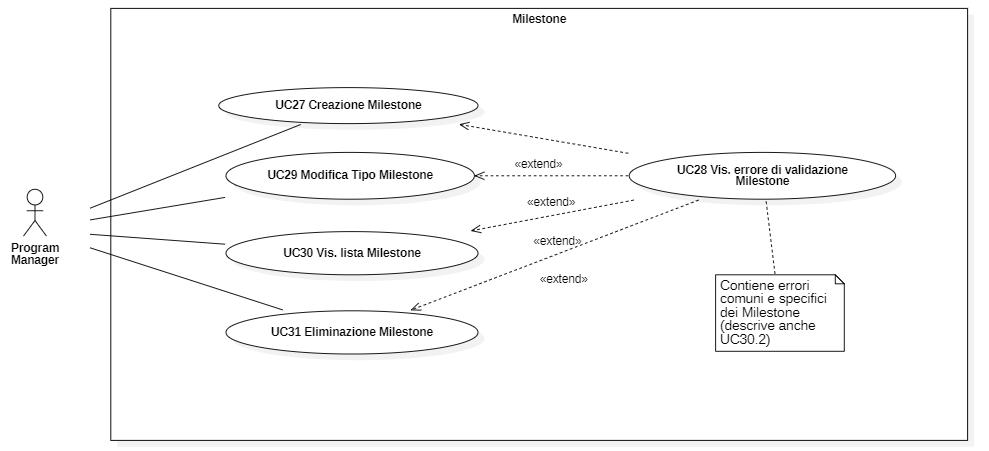
\includegraphics[width=1.05\columnwidth]{usecase/milestone-general} 
    \caption{Casi d'Uso del scenario Milestone}
\end{figure}

\subsubsection*{UC27 - Creazione Milestone}
\begin{itemize}[label=$\circ$]
\item \textbf{Attore:} Program Manager;
\item \textbf{Descrizione:} il Program Manager può creare una nuova Milestone da associare ad una Pianificazione;
\item \textbf{Precondizioni:} il richiedente è un Program Manager;
\item \textbf{Postcondizioni:} la Milestone è stata creata dal Program Manager con successo;
\item \textbf{Estensioni:} UC28;
\item \textbf{Inclusioni:} il caso d'uso non ha inclusioni.
\end{itemize}

\subsubsection*{UC28 - Vis. errore di validazione Milestone}
\begin{itemize}[label=$\circ$]
\item \textbf{Attore:} Program Manager;
\item \textbf{Descrizione:} questo caso d'uso descrive anche UC30.2. Viene visualizzato un messaggio di errore in caso vengano eseguite funzionalità con dati non validi. Esso rappresenta i seguenti errori comuni all'interno delle Milestone: dati non validi, filtri non valorizzati, entità associate non valide, risultati nulli o non valorizzati;
\item \textbf{Precondizioni:} il Program Manager sta effettuando operazioni con dati non validi;
\item \textbf{Postcondizioni:} l'esecuzione della funzionalità è interrotta e viene visualizzato il messaggio di errore;
\item \textbf{Estensioni:} il caso d'uso non ha estensioni;
\item \textbf{Inclusioni:} il caso d'uso non ha inclusioni.
\end{itemize}

\subsubsection*{UC29 - Modifica Tipo Milestone}
\begin{itemize}[label=$\circ$]
\item \textbf{Attore:} Program Manager;
\item \textbf{Descrizione:}  il Program Manager può modificare il Tipo di una Milestone in due possibili valori: Alert o Reminder;
\item \textbf{Precondizioni:} il richiedente è un Program Manager;
\item \textbf{Postcondizioni:} la Milestone è stata modificata con successo solo nel campo
Tipo dal Program Manager;
\item \textbf{Estensioni:} UC28;
\item \textbf{Inclusioni:} il caso d'uso non ha inclusioni.
\end{itemize}

\subsubsection*{UC30 - Vis. lista Milestone}
\begin{figure}[H] 
    \centering 
    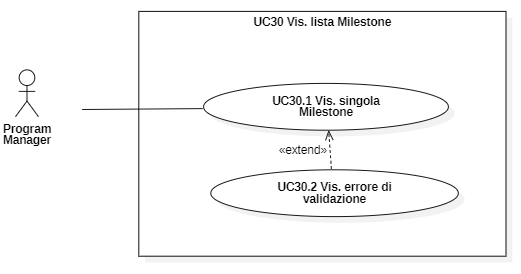
\includegraphics[width=0.70\columnwidth]{usecase/UC30} 
    \caption{Casi d'Uso 30 espanso}
\end{figure}
\begin{itemize}[label=$\circ$]
\item \textbf{Attore:} Program Manager;
\item \textbf{Descrizione:} il Program Manager può visualizzare una lista di Milestone dopo aver inserito filtri e/o una parola nella ricerca rapida e aver selezionato se i filtri applicati devono essere congiunti o disgiunti;
\item \textbf{Precondizioni:} il richiedente è un Program Manager;
\item \textbf{Postcondizioni:} la lista delle Milestone è visualizzabile dal Program Manager;
\item \textbf{Estensioni:} UC28;
\item \textbf{Inclusioni:} il caso d'uso non ha inclusioni.
\end{itemize}

\subsubsection*{UC30.1 - Vis. singola Milestone}
\begin{figure}[H] 
    \centering 
    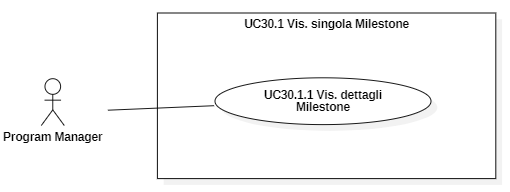
\includegraphics[width=0.70\columnwidth]{usecase/UC30.1} 
    \caption{Casi d'Uso 30.1 espanso}
\end{figure}
\begin{itemize}[label=$\circ$]
\item \textbf{Attore:} Program Manager;
\item \textbf{Descrizione:} il Program Manager può visualizzare la Milestone selezionata;
\item \textbf{Precondizioni:} la lista delle Milestone è visualizzabile;
\item \textbf{Postcondizioni:} la Milestone selezionata è visualizzabile dal Program Manager;
\item \textbf{Estensioni:} UC30.2;
\item \textbf{Inclusioni:} il caso d'uso non ha inclusioni.
\end{itemize}

\subsubsection*{UC30.1.1 - Vis. dettagli Milestone}
\begin{itemize}[label=$\circ$]
\item \textbf{Attore:} Program Manager;
\item \textbf{Descrizione:} il Program Manager può visualizzare la Milestone selezionata;
\item \textbf{Precondizioni:} la Milestone singola è visualizzabile;
\item \textbf{Postcondizioni:} il Project Manager può visualizzare i campi di una Milestone selezionata;
\item \textbf{Estensioni:} il caso d'uso non ha esclusioni;
\item \textbf{Inclusioni:} il caso d'uso non ha inclusioni.
\end{itemize}

\subsubsection*{UC31 - Eliminazione Milestone}
\begin{itemize}[label=$\circ$]
\item \textbf{Attore:} Program Manager;
\item \textbf{Descrizione:} il Program Manager può eliminare una Milestone esistente;
\item \textbf{Precondizioni:} il richiedente è un Program Manager;
\item \textbf{Postcondizioni:} la Milestone è stata eliminata dal Program Manager con successo;
\item \textbf{Estensioni:} UC28;
\item \textbf{Inclusioni:} il caso d'uso non ha inclusioni.
\end{itemize}



\section{Tracciamento dei requisiti}


 


    \chapter{Progettazione}
\label{cap:progettazione}

\section{Scopo del capitolo}
In questo capitolo si tratterà dei giorni successivi all'apprendimento del background tecnologico, in cui sono state improntate le basi dell'architettura del progetto, definendo inoltre uno schema iniziale del database su cui si poggerà l'API.\\
Nei seguenti paragrafi verrà quindi trattata l'architettura e le configurazioni utilizzate che funzionano da base per l'implementazione di quanto sviluppato.\\

\section{Configurazione del progetto}
\subsection{Spring Initializr}

\begin{figure}[!h] 
    \centering 
    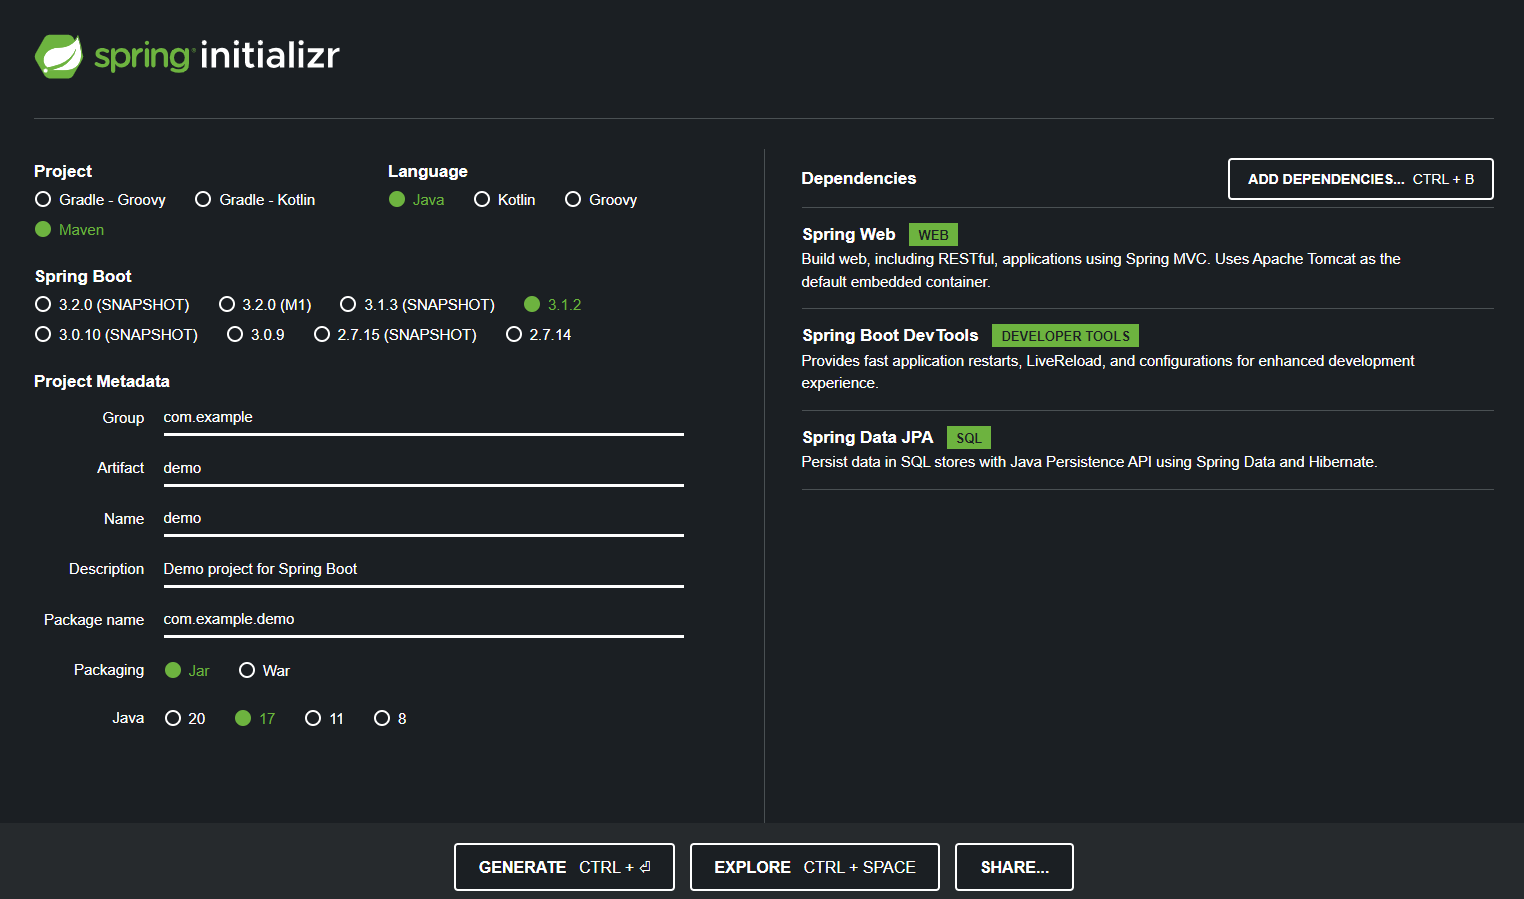
\includegraphics[width=0.95\columnwidth]{Spring_initializr} 
    \caption{Interfaccia Spring Initializr}
\end{figure}

\noindent \href{https://start.spring.io/}{Spring Initializr} è uno strumento online fornito dalla community di Spring Framework, che consente di creare rapidamente un progetto Spring Boot personalizzato, con le dipendenze e le configurazioni preselezionate dall'utente. Questo strumento semplifica notevolmente il processo di inizializzazione di un progetto Spring Boot, permettendo agli sviluppatori di risparmiare tempo e concentrarsi sulla scrittura del codice.\\
L'utente può selezionare il tipo di progetto di cui ha bisogno, come ad esempio un progetto Maven o Gradle, e specificare il linguaggio e la versione di Spring Boot desiderati. Inoltre, può anche inserire i metadati del progetto, come il nome del progetto e il nome dei packages.\\
Una volta selezionate le opzioni desiderate, l'utente può scegliere le dipendenze per il progetto. Le dipendenze sono librerie di terze parti che forniscono funzionalità aggiuntive al progetto.\\
Dopo aver selezionato le dipendenze, l'utente può scaricare il progetto Spring Boot personalizzato in formato ZIP. 

\subsection{File di configurazione}
Il file ZIP scaricato precedentemente contiene tutti i file necessari per iniziare a lavorare sul progetto, inclusi i file di configurazione.
Di seguito riporto il file pom.xml che si ottiene creando un progetto con le dipendenze sopra selezionate. La configurazione di Maven avviene proprio tramite questo file.\\
All'interno di questo file si possono trovare tag di questo tipo:
\begin{itemize}
\item \textbf{groupId}, organizzazione che ha creato il progetto;
\item \textbf{artifactId}, nome unico del progetto;
\item \textbf{version},  versione del progetto;
\item \textbf{packages}, un metodo in cui è salvato il progetto (JAR,WAR,ZIP,ecc…).
\end{itemize}

\noindent Nel file si possono notare le seguenti dipendenze:
\begin{itemize}
\item \textit{spring-boot-starter-web}, per utilizzare il framework Spring MVC per la creazione di applicazioni Web;
\item \textit{spring-boot-starter-jpa}, per la persistenza dei dati;
\item \textit{spring-boot-devtools}, offre tools per migliorare il processo di sviluppo come live reload e rilascio automatico;
\item \textit{spring-boot-starter-test}, per includere librerie di testing.
\end{itemize}
Rispetto al file utilizzato nel progetto mancano le seguenti dipendenze:
\begin{itemize}
\item \textit{Dipendenza 1}
\item \textit{Dipendenza 2}
\end{itemize}

\begin{lstlisting}[language=XML,caption = pom.xml con dipendenze selezionate]
<?xml version="1.0" encoding="UTF-8"?>
<project xmlns="http://maven.apache.org/POM/4.0.0" xmlns:xsi="http://www.w3.org/2001/XMLSchema-instance"
	xsi:schemaLocation="http://maven.apache.org/POM/4.0.0 https://maven.apache.org/xsd/maven-4.0.0.xsd">
	<modelVersion>4.0.0</modelVersion>
	<parent>
		<groupId>org.springframework.boot</groupId>
		<artifactId>spring-boot-starter-parent</artifactId>
		<version>3.1.2</version>
		<relativePath/> <!-- lookup parent from repository -->
	</parent>
	<groupId>com.example</groupId>
	<artifactId>demo</artifactId>
	<version>0.0.1-SNAPSHOT</version>
	<name>demo</name>
	<description>Demo project for Spring Boot</description>
	<properties>
		<java.version>17</java.version>
	</properties>
	<dependencies>
		<dependency>
			<groupId>org.springframework.boot</groupId>
			<artifactId>spring-boot-starter-data-jpa</artifactId>
		</dependency>
		<dependency>
			<groupId>org.springframework.boot</groupId>
			<artifactId>spring-boot-starter-web</artifactId>
		</dependency>

		<dependency>
			<groupId>org.springframework.boot</groupId>
			<artifactId>spring-boot-devtools</artifactId>
			<scope>runtime</scope>
			<optional>true</optional>
		</dependency>
		<dependency>
			<groupId>org.springframework.boot</groupId>
			<artifactId>spring-boot-starter-test</artifactId>
			<scope>test</scope>
		</dependency>
	</dependencies>

	<build>
		<plugins>
			<plugin>
				<groupId>org.springframework.boot</groupId>
				<artifactId>spring-boot-maven-plugin</artifactId>
			</plugin>
		</plugins>
	</build>

</project>
\end{lstlisting}


    \chapter{Analisi dei requisiti}
\label{cap:analisi-requisiti}

\intro{Breve introduzione al capitolo}\\

\section{Casi d'uso}

Per lo studio dei casi di utilizzo del prodotto sono stati creati dei diagrammi.
I diagrammi dei casi d'uso (in inglese \emph{Use Case Diagram}) sono diagrammi di tipo \gls{uml} dedicati alla descrizione delle funzioni o servizi offerti da un sistema, così come sono percepiti e utilizzati dagli attori che interagiscono col sistema stesso.
Essendo il progetto finalizzato alla creazione di un tool per l'automazione di un processo, le interazioni da parte dell'utilizzatore devono essere ovviamente ridotte allo stretto necessario. Per questo motivo i diagrammi d'uso risultano semplici e in numero ridotto.

\begin{figure}[!h] 
    \centering 
    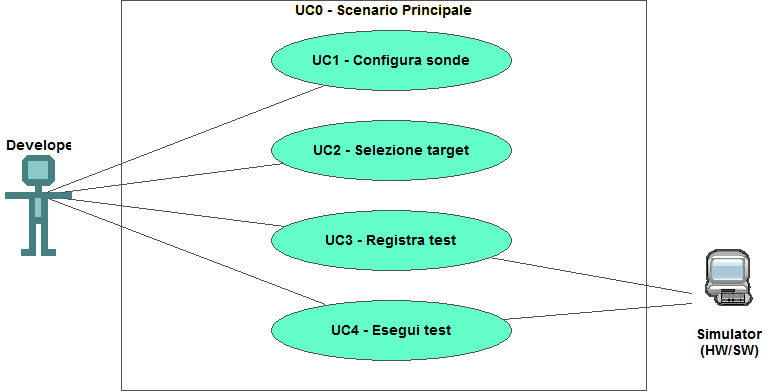
\includegraphics[width=0.9\columnwidth]{usecase/scenario-principale} 
    \caption{Use Case - UC0: Scenario principale}
\end{figure}

\begin{usecase}{0}{Scenario principale}
\usecaseactors{Sviluppatore applicativi}
\usecasepre{Lo sviluppatore è entrato nel plug-in di simulazione all'interno dell'IDE}
\usecasedesc{La finestra di simulazione mette a disposizione i comandi per configurare, registrare o eseguire un test}
\usecasepost{Il sistema è pronto per permettere una nuova interazione}
\label{uc:scenario-principale}
\end{usecase}

\section{Tracciamento dei requisiti}

Da un'attenta analisi dei requisiti e degli use case effettuata sul progetto è stata stilata la tabella che traccia i requisiti in rapporto agli use case.\\
Sono stati individuati diversi tipi di requisiti e si è quindi fatto utilizzo di un codice identificativo per distinguerli.\\
Il codice dei requisiti è così strutturato R(F/Q/V)(N/D/O) dove:
\begin{enumerate}
	\item[R =] requisito
    \item[F =] funzionale
    \item[Q =] qualitativo
    \item[V =] di vincolo
    \item[N =] obbligatorio (necessario)
    \item[D =] desiderabile
    \item[Z =] opzionale
\end{enumerate}
Nelle tabelle \ref{tab:requisiti-funzionali}, \ref{tab:requisiti-qualitativi} e \ref{tab:requisiti-vincolo} sono riassunti i requisiti e il loro tracciamento con gli use case delineati in fase di analisi.

\newpage

\begin{table}%
\caption{Tabella del tracciamento dei requisti funzionali}
\label{tab:requisiti-funzionali}
\begin{tabularx}{\textwidth}{lXl}
\hline\hline
\textbf{Requisito} & \textbf{Descrizione} & \textbf{Use Case}\\
\hline
RFN-1     & L'interfaccia permette di configurare il tipo di sonde del test & UC1 \\
\hline
\end{tabularx}
\end{table}%

\begin{table}%
\caption{Tabella del tracciamento dei requisiti qualitativi}
\label{tab:requisiti-qualitativi}
\begin{tabularx}{\textwidth}{lXl}
\hline\hline
\textbf{Requisito} & \textbf{Descrizione} & \textbf{Use Case}\\
\hline
RQD-1    & Le prestazioni del simulatore hardware deve garantire la giusta esecuzione dei test e non la generazione di falsi negativi & - \\
\hline
\end{tabularx}
\end{table}%

\begin{table}%
\caption{Tabella del tracciamento dei requisiti di vincolo}
\label{tab:requisiti-vincolo}
\begin{tabularx}{\textwidth}{lXl}
\hline\hline
\textbf{Requisito} & \textbf{Descrizione} & \textbf{Use Case}\\
\hline
RVO-1    & La libreria per l'esecuzione dei test automatici deve essere riutilizzabile & - \\
\hline
\end{tabularx}
\end{table}%

    \chapter{Progettazione e codifica}
\label{cap:progettazione-codifica}

\intro{Breve introduzione al capitolo}\\

\section{Tecnologie e strumenti}
\label{sec:tecnologie-strumenti}

Di seguito viene data una panoramica delle tecnologie e strumenti utilizzati.

\subsection*{Tecnologia 1}
Descrizione Tecnologia 1.

\subsection*{Tecnologia 2}
Descrizione Tecnologia 2

\section{Ciclo di vita del software}
\label{sec:ciclo-vita-software}

\section{Progettazione}
\label{sec:progettazione}

\subsubsection{Namespace 1} %**************************
Descrizione namespace 1.

\begin{namespacedesc}
    \classdesc{Classe 1}{Descrizione classe 1}
    \classdesc{Classe 2}{Descrizione classe 2}
\end{namespacedesc}


\section{Design Pattern utilizzati}

\section{Codifica}

    \chapter{Verifica e validazione}
\label{cap:verifica-validazione}

    \chapter{Conclusioni}
\label{cap:conclusioni}

Il mio percorso è iniziato con lo studio dei concetti di base e delle tecnologie che avrei utilizzato, sotto la guida del tutor Antonio Fasolato, prima di passare alle esercitazioni sulle tecnologie.\\
Tra le esercitazioni iniziali, quella su SpringBoot è risultata essere la più complessa. Essendo concetti nuovi che andavo ad affrontare, come l'utilizzo delle annotazioni di SpringBoot, non è stato semplice all’inizio comprendere il funzionamento del framework e questo ha portato ad un maggior investimento di tempo rispetto alle altre esercitazioni. È stato comunque un investimento proficuo poichè ha permesso di formarmi al meglio sulla tecnologia principale e alla base di quello che andavo a sviluppare.\\
Per poter comprendere al meglio ciò che andavo a creare, è stato svolto un incontro iniziale con il Senior Technical Leader Giovanni Incammicia, che mi ha illustrato le funzionalità del progetto dal lato Front-End. Successivamente è stato quindi deciso di definire le basi del mio prodotto, iniziando dal database e dallo scheletro delle risposte e delle richieste utilizzate dall’API REST.\\
Come linea guida è stato utilizzato un disegno iniziale dell’API e un'Analisi dei Requisiti fornita che comprendeva anche il lato Front-End.\\
Da qui è cominciato il mio lavoro sullo sviluppo delle nuove tabelle del database su cui poggiava l’API, integrandole con le tabelle aziendali fino allo sviluppo delle risposte e delle richieste che l’API utilizzava per ogni funzionalità.\\
Le ultime attività effettuate sono state il testing e la validazione di quanto sviluppato. Tuttavia, lo sviluppo delle funzionalità ed eventuali problematiche implementative, hanno ridotto il tempo disponibile per il testing. Di conseguenza, sebbene sia stato affrontato in modo adeguato a livello teorico, non è stato possibile implementarlo pienamente, come evidenziato nella sezione di \hyperlink{testing}{Testing}.

\section{Consuntivo finale}
L’attività di tirocinio è durata 320 ore, come preventivato nel piano di lavoro, iniziando il 19 Giugno e finendo il 24 Agosto. La ripartizione delle ore mostrata nel piano di lavoro, anche se indicativa, è stata abbastanza rispettata.\\
Inizialmente, le esercitazioni sono state spalmate in modo adeguato nelle prime settimane. Successivamente, il tempo dedicato alla progettazione è stato utilizzato completamente, mentre il tempo riservato al testing non è stato sufficiente, a causa delle problematiche riscontrate nello sviluppo dell'API dovute all'adozione di tecnologie poco conosciute, che hanno causato rallentamenti.

\section{Principali problematiche e soluzioni}
\subsection*{Problematiche}
\begin{enumerate}
\item Per cominciare lo sviluppo del progetto è stata presa come base un’Analisi dei Requisiti del progetto completo (lato Front-end integrato con lato Back-end) insieme ad una bozza dell'API che dovevo andare a sviluppare. È stato dunque difficile riuscire a far concordare quello che l’API suggeriva di implementare con il requisito completo che l’Analisi dei Requisiti forniva ed arrivare al codice da sviluppare;
\item Le funzionalità che ho implementato richiedevano l'accesso a dati recuperati da tabelle da me create. Tuttavia queste tabelle necessitavano di dati da altre tabelle già esistenti nel database aziendale. La problematica era quella di identifcare quali tabelle del database aziendale dovevo collegare alle tabelle di mia creazione; 
\item Nel periodo finale di tirocinio mi sono interfacciato con chi lavorava nel lato Front-End per poter cominciare ad integrare il mio lavoro ed avere una visione più completa di quanto implementato. Per poter fare questo bisognava quindi avere una documentazione dell’API chiara e concordata tra le parti.
\end{enumerate}

\subsection*{Soluzioni}
\begin{enumerate}
\item Per lo sviluppo è stato preso in considerazione il mock iniziale dell’API , utilizzando come consulto per un chiarimento sulla funzionalità fornita dall’endpoint, l’Analisi dei Requisiti, come spiegato nella sezione di \hyperlink{validation}{Validazione}. A fine del tirocinio è stata poi creato un nuovo documento dell'API, come descritto nella sezione dello \hyperlink{swagger}{Swagger} nel capitolo di Sviluppo dell’API REST, considerandolo come documento unico per la consultazione dell’API sviluppata;
\item Per avere una comprensione migliore del database aziendale mi è stato fornito un backup del database di testing aziendale con dati fittizi in cui c’era la possibilità di testare come volevo. Grazie al tutor e agli altri collaboratori ho avuto una visione più completa di come funzionasse il database aziendale e a quali tabelle dovevo fare riferimento;
\item Per poter comunicare correttamente con gli altri sviluppatori è stato creato il file Swagger. Tuttavia, come spiegato nel capitolo di \hyperlink{validation}{Validazione}, a fine progetto, anche se l’API era chiara e documentata, ci sono state delle discrepanze tra le funzionalità implementate che non hanno permesso la fase di Collaudo.
\end{enumerate}

\section{Analisi critica del prodotto}
\subsection{Utilizzo del prodotto}
Il prodotto sviluppato verrà integrato con la parte di Front-End in seguito ad un refactoring del codice e all'aggiunta delle funzionalità mancanti da chi di dovere. Le tabelle da me create verranno integrate al database aziendale per permettere la fruizione dei servizi dell'API.\\ In seguito all'integrazione delle funzionalità il prodotto sarà disponibile all'utilizzo da parte dei Project Manager e dei Program Manager per semplificare la creazione di richieste e di pianificazioni di risorse aziendali.

\subsection{Valutazione strumenti utilizzati}
\subsubsection*{Spring}
L'utilizzo delle annotazioni per fornire un significato preciso, introducendo quindi il design pattern Inversion of Control, e l'iniezione di alcuni componenti all'interno di altri, mi ha messo in difficoltà all'inizio del progetto, rallentando la fase di sviluppo.
Un elemento che mi ha colpito dell'adozione di Spring è stato come andasse a recuperare le configurazioni di ogni componente e, una volta capito al meglio la funzionalità del framework, quanto fosse facile aggiungerne.

\subsubsection*{Spring Data}
Mi ha particolarmente colpito Spring Data JPA e le interfacce che offre, come ad esempio \textit{JpaRepository}. All'inizio, comprendere che questa interfaccia consentisse di eseguire operazioni CRUD personalizzate nel database tramite parole chiave non è stato semplice. Tuttavia, una volta acquisita familiarità con questa tecnologia, ho realizzato quanto semplificasse l'accesso al database.

\subsubsection*{Swagger}
Strumento utilizzato per rappresentare lo sviluppo della mia API. Sono rimasto soddisfatto della completezza dello strumento e della chiarezza della sua interfaccia grafica. All'inizio del progetto, questa chiarezza mi ha aiutato a comprendere al meglio la composizione delle risposte e delle richieste di ogni endpoint del mock dell'API fornito.

\subsection{Completamento dei Requisiti}
Le funzionalità principali dell’API sono state sviluppate tutte permettendoci di arrivare ad un prodotto funzionante. Tuttavia alcuni requisiti, per mancanza di tempo, non sono stati sviluppati perchè ritenuti meno importanti o perchè necessitavano di tempo che non avevamo più a disposizione. Ad esempio …

\subsection{Possibili estensioni}
Il mio prodotto non è completo e sicuramente mancano alcune funzionalità che lo porterebbero ad essere un prodotto migliore.\\
Le possibili estensioni possono essere:
\begin{itemize}
\item un refactoring del codice per agevolare il riutilizzo del codice;
\item implementazione di servizi esterni per la raccolta di informazioni sulle risorse aziendali;
\item calcolo delle date di fine o dei giorni in base alla disponibilità delle risorse, interfacciandosi con ulteriori software di gestione delle risorse umane o delle attività.
\end{itemize} 

\section{Conoscenze acquisite}
Le conoscenze acquisite in questi anni universitari hanno agevolato di molto la comprensione delle nuove tecnologie che sono andato a studiare. Ritengo di aver acquisito, in seguito a questa esperienza, conoscenze soddisfacenti verso le tecnologie elencate nel capitolo di \hyperlink{tecnologie}{Background Tecnologico}, con particolare rilevanza sottolineo: SpringBoot, Spring Data, Postman e Swagger.

\section{Valutazione personale}
Al termine di questa attività, mi ritengo soddisfatto e felice di aver intrapreso un'esperienza di questo tipo. Questa opportunità mi ha aiutato a comprendere come funziona un'azienda nel campo dell'informatica, ma soprattutto mi ha messo alla prova sulle mie conoscenze, contribuendo a consolidarle.\\
Anche se sono contento di ciò che ho sviluppato e imparato, mi rammarico di non essere riuscito ad osservare direttamente l'integrazione tra ciò che ho implementato io e il Front-End.\\
Ringrazio il mio tutor, Antonio Fasolato, per la sua disponibilità, pazienza e dedizione nel farmi comprendere concetti a me sconosciuti, incoraggiandomi ad affrontare tutti i problemi cercando di farmi trovare la soluzione da solo prima di fornirmela.\\
Ringrazio inoltre tutte le persone che ho conosciuto all'interno dell'azienda, apprezzando molto l'accoglienza ricevuta e l'atmosfera che si respirava in azienda.\\
Considero questa opportunità un'esperienza ottima per il concludere il mio percorso di laurea e ringrazio l'Università e l'azienda Omicron Consulting della possibilità.


    \appendix
    \chapter{Appendice A}

\epigraph{Citazione}{Autore della citazione}

    \backmatter
    \printglossary[type=\acronymtype, title=Acronimi e abbreviazioni, toctitle=Acronimi e abbreviazioni]
    \printglossary[type=main, title=Glossario, toctitle=Glossario]

    \cleardoublepage
\chapter{Bibliografia}

\nocite{*}

% Print book bibliography
\printbibliography[heading=subbibliography,title={Riferimenti bibliografici},type=book]

% Print site bibliography
\printbibliography[heading=subbibliography,title={Siti web consultati},type=online]

\begin{itemize}
\item https://it.wikipedia.org/wiki/Java\_(linguaggio\_di\_programmazione)
\item https://docs.spring.io/spring-framework/reference/overview.html
\item https://spring.io/projects/spring-boot
\item https://spring.io/projects/spring-data
\item https://it.wikipedia.org/wiki/Structured\_Query\_Language
\item https://www.json.org/json-it.html
\item https://it.wikipedia.org/wiki/IntelliJ\_IDEA
\item https://www.baeldung.com/maven
\item https://en.wikipedia.org/wiki/DBeaver
\item https://it.wikipedia.org/wiki/Microsoft\_SQL\_Server
\item https://www.baeldung.com/spring-boot-hibernate
\item https://learning.postman.com/docs/introduction/overview/
\item https://it.wikipedia.org/wiki/Microsoft\_Teams
\item https://en.wikipedia.org/wiki/Notion\_(productivity\_software)
\item https://it.wikipedia.org/wiki/Microsoft\_Excel
\item https://it.wikipedia.org/wiki/Visual\_Studio\_Code
\item https://it.wikipedia.org/wiki/Docker
\item https://swagger.io/docs/specification/about/
\item https://git-scm.com/docs/git
\item https://it.wikipedia.org/wiki/GitLab
\item http://gitextensions.github.io/
\item https://it.wikipedia.org/wiki/Front\_Controller\_pattern

\end{itemize}
\end{document}
